\documentclass{article}
\usepackage{fancyhdr}
\usepackage{ctex}
\usepackage[a4paper, body={18cm,22cm}]{geometry}
\usepackage{amsmath,amssymb,amstext,wasysym,enumerate,graphicx}
\usepackage{float,abstract,booktabs,indentfirst,amsmath}
\usepackage{multirow}
\usepackage{enumitem}
\usepackage{xcolor}
\usepackage{tabularx}
\usepackage[most]{tcolorbox}
\usepackage{accsupp}
\usepackage[bottom]{footmisc}
\usepackage{subcaption}
\usepackage{logicproof}
% \usepackage[backend=biber,style=numeric]{biblatex}
\usepackage[xetex]{hyperref}
\usepackage{fontspec}
\usepackage{listingsutf8}
\usepackage{xcolor}
\usetikzlibrary{arrows.meta}
\newcommand\emptyaccsupp[1]{\BeginAccSupp{ActualText={}}#1\EndAccSupp{}}
\setlength{\parindent}{2em}
\setmonofont{Consolas}
\setCJKmonofont{黑体}
% \setmainfont{Times New Roman}
\hypersetup{CJKbookmarks=true,colorlinks=true,citecolor=blue,%
            linkcolor=blue,urlcolor=blue,bookmarksnumbered=true,%
            bookmarksopen=true,breaklinks=true}
\lstset{
    % language = C,
    inputencoding=utf8,
    extendedchars=false,
    showstringspaces=false,
    xleftmargin = 3em,xrightmargin = 3em, aboveskip = 1em,
	backgroundcolor = \color{white}, % 背景色
	basicstyle = \small\ttfamily, % 基本样式 + 小号字体
	rulesepcolor= \color{gray}, % 代码块边框颜色
	breaklines = true, % 代码过长则换行
	numbers = left, % 行号在左侧显示
	numberstyle=\emptyaccsupp,
    numbersep = 14pt, 
    keywordstyle=\color{purple}\bfseries, % 关键字颜色
    commentstyle =\color{red!50!green!50!blue!60}, % 注释颜色
    stringstyle = \color{red}, % 字符串颜色
    morekeywords={ASSERT, int64_t, uint32_t},
	% frame = shadowbox, % 用(带影子效果)方框框住代码块
	frame = single, % 用(带影子效果)方框框住代码块
	showspaces = false, % 不显示空格
	columns = fixed, % 字间距固定
  framesep=1em
} 
\lstset{
    sensitive=true,
    moreemph={ASSERT, NULL}, emphstyle=\color{red}\bfseries,
    moreemph=[2]{int64_t, uint32_t, tid_t, uint8_t, int16_t, uint16_t, int32_t, size_t}, emphstyle=[2]\color{purple}\bfseries,
    showspaces = false, % 不显示空格
    }

\raggedbottom

\title{\heiti\textbf{机器学习实践报告}}
\author{第一次实验 \\ 
武泽恺 10225101429
}
\date{2025年10月19日}

\begin{document}
\maketitle

\section{实验目的}
\begin{itemize}
  \item 掌握 numpy、pandas 与 matplotlib 库的基本使用方法。
  \item 能够进行基础的数据创建、索引、运算和可视化。
\end{itemize}

\section{实验环境}
\begin{itemize}
  \item Python 版本:3.x
  \item 使用库:numpy、pandas、matplotlib
\end{itemize}

\section{实验内容与代码}

\subsection{创建与操作数组}
\begin{lstlisting}[language=Python]
A = np.arange(1, 11)
B = np.random.randint(1, 100, (4, 5))
A_T = A.reshape(-1, 1)
B_plus = B + 1
\end{lstlisting}

\begin{figure}[H]
  \centering
  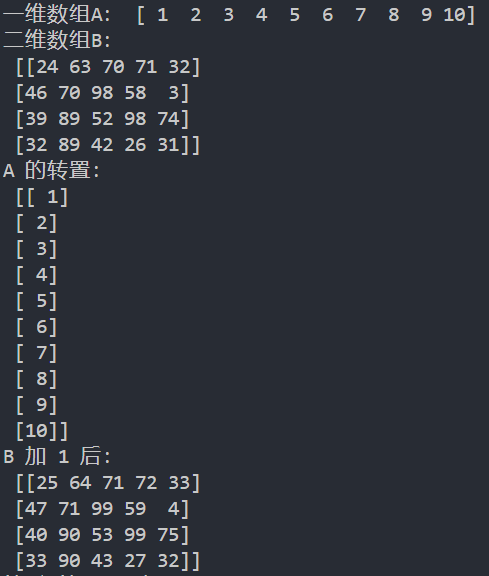
\includegraphics[width=0.6\textwidth]{image.png}
  \caption{实验内容1}
\end{figure}

\subsection{数组索引与切片}
\begin{lstlisting}[language=Python]
B[1, 2]
B[1, :]
B[:, 2]
B[:2, :2]
\end{lstlisting}

\begin{figure}[H]
  \centering
  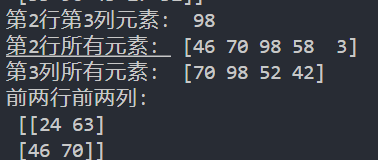
\includegraphics[width=0.6\textwidth]{image1.png}
  \caption{实验内容2}
\end{figure}

\subsection{数组运算}
\begin{lstlisting}[language=Python]
A2 = np.arange(10, 20)
A + A2
row_mean = np.mean(B, axis=1)
\end{lstlisting}

\begin{figure}[H]
  \centering
  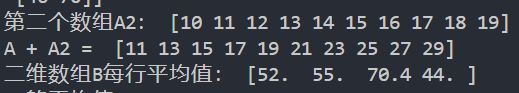
\includegraphics[width=0.6\textwidth]{image2.png}
  \caption{实验内容3}
\end{figure}

\subsection{使用 numpy 函数}
\begin{lstlisting}[language=Python]
np.mean(A)
np.std(A)
np.sort(A)
\end{lstlisting}

\begin{figure}[H]
  \centering
  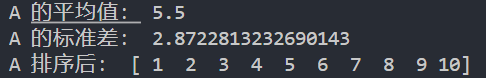
\includegraphics[width=0.6\textwidth]{image3.png}
  \caption{实验内容4}
\end{figure}

\subsection{复杂数据分析}

\begin{lstlisting}[language=Python]
df = pd.read_excel("score.xlsx")
df.iloc[:, 0] = df.iloc[:, 0].astype(str)
student_id = input("请输入学号:").strip()
student = df[df.iloc[:, 0] == student_id]
labels = df.columns[1:]
scores = student.iloc[0, 1:].values
num_labels = len(labels)

angles = np.linspace(0, 2 * np.pi, num_labels, endpoint=False).tolist()
scores = np.concatenate((scores, [scores[0]]))
angles += angles[:1]
plt.figure()
plt.polar(angles, scores, 'o-', linewidth=2)
plt.fill(angles, scores, alpha=0.25)
plt.xticks(angles[:-1], labels)
plt.title(f"{student_id} 成绩雷达图")
plt.show()

df["总分"] = df.iloc[:, 1:].sum(axis=1)
top6 = df.nlargest(6, "总分")
plt.figure()
plt.bar(top6.iloc[:, 0], top6["总分"])
plt.xlabel("学号")
plt.ylabel("总分")
plt.title("总分前6名")
for i, v in enumerate(top6["总分"]):
    plt.text(top6.iloc[i, 0], v + 1, str(v), ha='center')
plt.show()

course = input("课程名称:")
grades = df[course]
categories = ["优秀", "良好", "中等", "及格", "不及格"]
counts = [
    ((grades >= 90) & (grades <= 100)).sum(),
    ((grades >= 80) & (grades < 90)).sum(),
    ((grades >= 70) & (grades < 80)).sum(),
    ((grades >= 60) & (grades < 70)).sum(),
    (grades < 60).sum()
]
plt.figure()
plt.pie(counts, labels=categories, autopct="%.1f%%", startangle=90)
plt.show()
\end{lstlisting}

\begin{figure}[H]
  \centering
  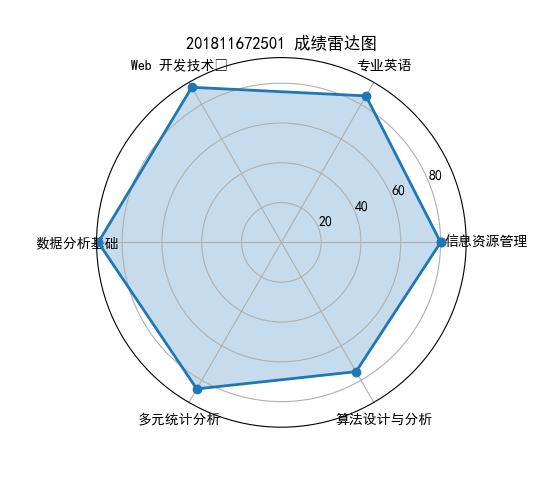
\includegraphics[width=0.6\textwidth]{Figure_0.png}
  \caption{实验内容5-1}
\end{figure}

\begin{figure}[H]
  \centering
  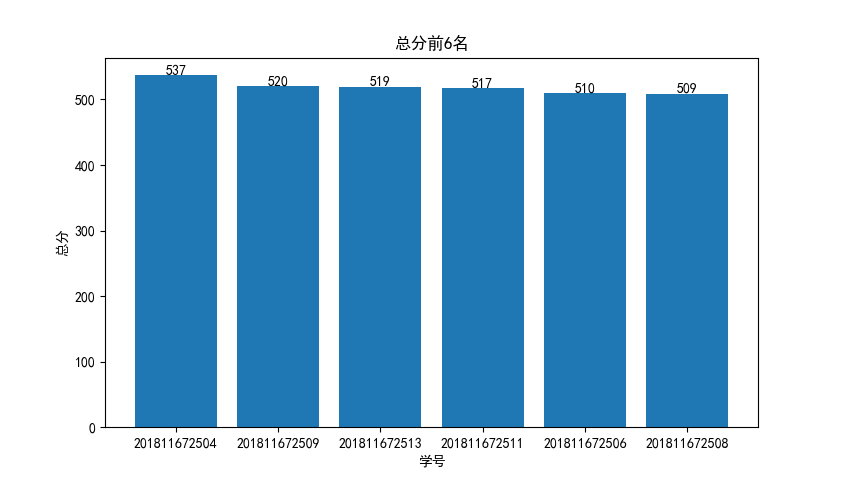
\includegraphics[width=0.6\textwidth]{Figure_1.png}
  \caption{实验内容5-2}
\end{figure}


\begin{figure}[H]
  \centering
  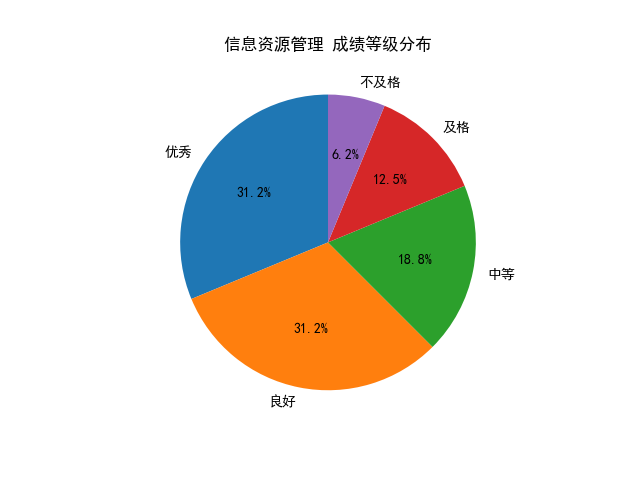
\includegraphics[width=0.6\textwidth]{Figure_2.png}
  \caption{实验内容5-3}
\end{figure}


\section{实验结果分析}

我们可以看到,程序运行结果显示:
\begin{itemize}
  \item 成功创建数组并进行索引与运算;
  \item 正确绘制雷达图、柱形图与饼状图;
  \item 数据分析与可视化呈现正确结果。
\end{itemize}

\section{实验总结}
通过本实验,熟悉了 numpy 的数组操作、pandas 的数据处理以及 matplotlib 的可视化绘制。  
掌握了基础数据分析的完整流程。

\end{document}